%% LaTeX2e class for student theses
%% thesis.tex
%% 
%% Karlsruhe Institute of Technology
%% Institute for Program Structures and Data Organization
%% Chair for Software Design and Quality (SDQ)
%%
%% Dr.-Ing. Erik Burger
%% burger@kit.edu
%%
%% See https://sdq.kastel.kit.edu/wiki/Dokumentvorlagen
%%
%% Version 1.3.6, 2022-09-28

%% Available page modes: oneside, twoside
%% Available languages: english, ngerman
%% Available modes: draft, final (see README)
\documentclass[oneside, english]{sdqthesis}

%% ---------------------------------
%% | Information about the thesis  |
%% ---------------------------------

%% Name of the author
\author{Violina Zhekova}

%% Title (and possibly subtitle) of the thesis
\title{Detecting Ambiguity in Neural Machine Translation Models by Inspecting Diversity in Translation}

%% Type of the thesis 
\thesistype{Master's Thesis}

%% Change the institute here, ``KASTEL'' is default
\myinstitute{Artificial Intelligence for Language Technologies (AI4LT)}

%% You can put a logo in the ``logos'' directory and include it here
%% instead of the SDQ logo
% \grouplogo{myfile}
%% Alternatively, you can disable the group logo
\nogrouplogo

%% The reviewers are the professors that grade your thesis
\reviewerone{Prof. Dr. Jan Niehues}
\reviewertwo{Prof. Dr. Alexander Waibel}

%% The advisors are PhDs or Postdocs
\advisorone{M. Sc. Tu Anh Dinh}

%% Please enter the start end end time of your thesis
\editingtime{01. May 2023}{02. November 2023}

\settitle

%% --------------------------------
%% | Bibliography                 |
%% --------------------------------

%% Use biber instead of BibTeX, see README
% style=authoryear; without numbers in Bibliography
\usepackage[style=numeric, citestyle=authoryear, maxbibnames=15, maxcitenames=2, abbreviate=false, backend=biber, natbib=true]{biblatex}
\addbibresource{thesis.bib}

%% ====================================
%% ====================================
%% ||                                ||
%% || Beginning of the main document ||
%% ||                                ||
%% ====================================
%% ====================================
\begin{document}

%% Set PDF metadata
\setpdf

%% Set the title
\maketitle

%% The Preamble begins here
\frontmatter

\thispagestyle{empty}
\null\vfill
\noindent\hbox to \textwidth{\hrulefill} 
\iflanguage{english}{I declare that I have developed and written the enclosed
thesis completely by myself. I have submitted neither parts of nor the complete 
thesis as an examination elsewhere. I have not used any other than the aids that
I have mentioned. I have marked all parts of the thesis that I have included from 
referenced literature, either in their original wording or paraphrasing their
contents. This also applies to figures, sketches, images and similar depictions,
as well as sources from the internet.}%
{Ich versichere hiermit, dass ich die vorliegende Arbeit selbstständig verfasst,
und weder ganz oder in Teilen als Prüfungsleistung vorgelegt und keine anderen
als die angegebenen Hilfsmittel benutzt habe. Sämtliche Stellen der Arbeit, die
benutzten Werken im Wortlaut oder dem Sinn nach entnommen sind, habe ich durch
Quellenangaben kenntlich gemacht. Dies gilt auch für Zeichnungen, Skizzen,
bildliche Darstellungen und dergleichen sowie für Quellen aus dem Internet. }
 
 
%% ---------------------------------------------
%% | Replace PLACE and DATE with actual values |
%% ---------------------------------------------
\textbf{PLACE, DATE}
\vspace{1.5cm}
 
\dotfill\hspace*{8.0cm}\\
\hspace*{2cm}(\theauthor) 
\cleardoublepage

\setcounter{page}{1}
\pagenumbering{roman}

%% ----------------
%% |   Abstract   |
%% ----------------
 
%% For theses written in English, an abstract both in English
%% and German is mandatory.
%%
%% For theses written in German, a German abstract is sufficient.
%%
%% The text is included from the following files:
%% - sections/abstract

\includeabstract

%% ------------------------
%% |   Table of Contents  |
%% ------------------------
\tableofcontents

\listoffigures
\listoftables

%% -----------------
%% |   Main part   |
%% -----------------

\mainmatter

\chapter{Introduction}
\label{ch:Introduction}

% Title: Detecting Ambiguity in Neural Machine Translation Models by Inspecting Diversity in Translation

% PRICoBE:
% Problem: What is the problem you are trying to address?
% Research questions: What are the research questions you are trying to answer? (to make novelty/originality clear)
% Idea: What is your idea of how to address the problem? (is often broader than the contribution)
% Contributions: Which contributions to the research area are you making with that idea?
% Benefits: What are the benefits of your contributions?
% Evaluation: How do you plan to evaluate your envisioned benefits? (Validation)

% Define clear research objectives: Clearly define the goals and objectives of your research. These objectives should be specific, measurable, achievable, relevant, and time-bound (SMART).


% Introduce ML, MT, NMT
In the world more than 7000 natural languages are spoken nowadays. It is humanly impossible to learn every language, which outlines the need for translation between different languages for the purpose of communication. This is a task for Machine Translation (MT), a subfield of Machine Learning (ML) that focuses on automatic translation from one language to another using computer technology. Machine Translation (MT) technology has assisted humans in gathering, processing, and communicating information.  

%%%%%%%%%%%%%%%%%%%%%%%%%%%%%%%%%%%%%%%%%%%%%%%%%%%%%%%%%%%%%%%%%%%%%%%%%%%%%%%%%%%%%%%%%%%%
\section{Motivation}
\label{sec:Introduction:Motivation}

% Elaborate on the problem of bias and ambiguity (interplay of bias and ambiguity) and how it affects different individuals
The development of Artificial Intelligence (AI) in recent years has expanded the field of MT and made it possible for people from all over the world to connect, learn and work in a foreign language. One application of AI is Neural Machine Translation (NMT), which uses deep learning to learn a statistical neural model for machine translation in an end-to-end fashion, translating directly from an input source language to an output target language. Neural networks (NNs) are typically trained on large corpora of natural occurring data extracted from the internet \parencite{NMT}. 
One problem with this data is it often contains social constructs and stereotypes. As a consequence, NMT models learn the biases from the data and perpetuate them, affecting downstream applications like coreference resolution \parencite{Zhao_2018_coreference} and contributing further to discrimination based on gender, race, age and religious beliefs \parencite{Rudinger_2017}. Some examples of this phenomenon include stereotyping professions, e.g. associating doctors with men and nurses with women \parencite{Escud_Font_2019}, and stereotyping behaviors, e.g. associating women with gossiping and men with guitars \parencite{Rudinger_2017}. Stereotypical assumptions in turn tend to impact individuals' perceptions of reality and influence their behavior in accordance with stereotypical expectations.

%%%%%%%%%%%%%%%%%%%%%%%%%%%%%%%%%%%%%%%%%%%%%%%%%%%%%%%%%%%%%%%%%%%%%%%%%%%%%%%%%%%%%%%%%%%%
\section{Research Questions}
\label{sec:Introduction:Questions}

% State objective
The objective of this work is to develop a method to detect ambiguous words in written text by inspecting the diversity of translation. In order to achieve this, I attempt to answer the following questions systematically.

\paragraph{Main research question: } How can we detect ambiguous words in translated written text?
\begin{itemize}
    \item How diverse are translations? % inspecting diversity patterns in translations which could point to ambiguity
    \item How does language influence the discovery of ambiguity? % different language families and alphabets may have different effect on translation ambiguous words
    \item How does context influence the discovery of ambiguity? 
\end{itemize}

% TODO: mention the type of ambiguity I am detecting

%%%%%%%%%%%%%%%%%%%%%%%%%%%%%%%%%%%%%%%%%%%%%%%%%%%%%%%%%%%%%%%%%%%%%%%%%%%%%%%%%%%%%%%%%%%%
\section{Contribution}
\label{sec:Introduction:Contribution}

As a part of the thesis, I want to contribute to solving the problem of bias in Machine Translation by developing an approach for detecting ambiguous words that could lead to bias. 
% TODO: Summarize approach, evaluation method and results 

In recent years, light has been shed on the different types of biases present in Neural Machine Translation (NMT) systems, the most researched type being gender bias \parencite{Savoldi_2021}. Some previous works have attempted to uncover gender bias in existing systems \parencite{Prates_2019}, while others have tried mitigating gender bias by either modifying the data (e.g. \cite{Escud_Font_2019}, \cite{Stanovsky_2019}) or changing the architecture of the system \parencite{Vanmassenhove_2018}. While there have been some studies on finding biases in MT, this is the first study aiming to create a framework for detecting ambiguity in a text, which contains no contextual information relating to the ambiguity, therefore making several translations possible. The ability to uncover ambiguity could in turn help to alleviate the problem of MT systems making an unjustified assumption, leading to bias.


%%%%%%%%%%%%%%%%%%%%%%%%%%%%%%%%%%%%%%%%%%%%%%%%%%%%%%%%%%%%%%%%%%%%%%%%%%%%%%%%%%%%%%%%%%%%
\section{Thesis Outline}
\label{sec:Introduction:Outline}
The rest of the thesis is structured as follows. Chapter 2 describes the background of NMT systems and introduces the problems stemming from language ambiguity and bias in the data. Next, Chapter 3 introduces some existing research on the topic, such as techniques to detect, assess, and mitigate bias in MT. Chapter 4 states the research problem and describes approaches used to answer the research questions. Furthermore, Chapter 5 describes the design of the experiments performed, which includes the corpora, models and evaluation methods used to conduct the experiments as well as technical details necessary for reproducibility. In Chapter 6 the results of the experiments are presented and discussed. Chapter 7 outlines the answers to the research questions from conducting the experiments and discusses challenges and limitations. Finally, Chapter 8 summarizes the key findings and proposes possible directions for future work.
\chapter{Background}
\label{ch:Background}


\section{Neural Machine Translation}
\label{sec:Background:NMT}

%TODO: sources
Machine Translation (MT) is the process of using computer technology to translate text from one natural language to another. This can be achieved using different paradigms. There are three main types of machine translation systems: Rule-based Machine Translation (RBMT), Statistical Machine Translation (SMT). 

Conventional RBMT systems use pre-defined rules based on syntax, morphology and semantics, created by professional linguists. However, the key weakness of rule-based translation systems is that they require extensive lexicons and a large set of rules. 

SMT systems, on the other hand, uses a data-driven approach that utilizes statistical models derived from the analysis of bilingual and monolingual corpora. The quality of SMT output depends heavily on the size and quality of the corpora used to train the models.

Neural Machine Translation (NMT) is a subfield of SMT, which uses an artificial neural network to learn a statistical model for machine translation. Unlike traditional SMT systems, which require a pipeline of specialized components such as language model and translation model, NMT trains its statistical model end-to-end, mapping directly from an input source language to an output target language. NMT can recognize patterns in the source material to determine a context-based interpretation that can predict the likelihood of a sequence of words. They are more memory-efficient than SMT models and also have a higher accuracy, which makes them the appropriate choice for creating high-quality MT systems.

%TODO: figure, sources
The architecture of NMT models often consists of an encoder and a decoder
(Figure 1). Firstly, each word in the input sentence is fed separately into the
encoder to encode the source sentence into an internal fixed-length representation
called the context vector. This context vector contains the meaning of the sentence.
Secondly, the decoder decodes the fixed-length context vector and then predicts
the output sequence. While some types of Encoder-Decoder model used LSTM-based
approach (e.g. Sutskever et al. (2014), Luong et al. (2015b)), the others (e.g.
Luong et al. (2015a), Vaswani et al. (2017), Galassi et al. (2019)) explored the use of attention-based architectures for neural machine translation. Since in this work, I make use of models based on the Transformer architecture, next I will introduce its basic principle and components.

%TODO: figure and sources
\paragraph{Transformer architecture} 
A Transformer is an Encoder-Decoder Sequence-to-Sequence model, introduced by \cite{transformer}. Sequence-to-Sequence models consist of an Encoder and a Decoder. The Encoder takes the input sequence and maps it into a higher dimensional space, an n-dimensional matrix, that contains token embeddings for each token of the sequence, carrying context information about the other tokens in the sequence weighted by relevance. That abstract matrix is fed into the Decoder, which produces an output sequence by autoregressive sampling from the encoder matrix and its own previous values. An important feature of the Transformer architecture is its attention mechanism. The attention module looks at an input sequence and decides at each step which other parts of the sequence are important, differentially weighting the significance of each part of the input data. 

Like Recurrent Neural Networks (RNNs), Transformers are designed to handle sequential input data, such as natural language. However, unlike RNNs, Transformers can process the whole input sequence in parallel. The attention mechanism provides context for any position in the input sequence. This feature allows for more parallelization than RNNs and therefore reduces training times significantly.

% HOW in deep should I explain the Transformer and NMT
- Transformer and deep learning
- Word embeddings
- WSD (if I end up using it)
- Definitions of bias and  ambiguity
- Types of biases
- Types of languages

\section{Ambiguity and Bias in Machine Translation}
\label{sec:Background:Ambiguity_Bias}

Biases present in AI systems are an important problem stemming from cultural and historical issues present in the data from which models are learning. The developed systems in turn reinforce the present societal prejudices and old social norms, instead of mitigating them.

% “man is to computer programmer as woman is to homemaker” \parencite{bolukbasi2016man}


% For bias detection we need:
% - Challenge sets are artificially created usually small datasets that represent some gender-related issue, such as assigning the right pronoun to a specific role
% - Automatic evaluation methods needed, because the BLEU score, normally used for assessing the quality of translations, cannot judge on the occurrence of bias
% WSD: technique in natural language processing (NLP), defined as the ability to determine which meaning of word is activated by the use of word in a particular context
% QE: method for predicting the quality of a given translation rather than assessing how similar it is to a reference segment, E.g. multiple beams in Beam search: low confidence = high confidence for error in translation


\chapter{Related Work}
\label{ch:Related_work}

% Conduct a thorough literature review: Familiarize yourself with existing research and literature related to your topic. Identify the knowledge gaps and research questions that your thesis will address. 

% - summarize the existing work
% - discuss how the present work differs from it and why this is a “step forward” (new or better)

Previous scientific work around bias has focused on detection and mitigation of bias in NMT models using various techniques, which I will present in the following two sections.  % For more information, \citet{Savoldi_2021} provide a more extensive literature review on the topic of gender bias in MT, critically reviewing current conceptualizations of bias in light of theoretical insights from related disciplines. 

%%%%%%%%%%%%%%%%%%%%%%%%%%%%%%%%%%%%%%%%%%%%%%%%%
\section{Bias Detection}
\label{sec:Background:Bias_Detection}

Dedicated benchmarks, evaluations, and experiments have been designed in order to assess the existence and scale of gender bias across several languages. In MT, several studies concerned themselves with pronoun translation and coreference resolution across typologically different languages. 

For example, \citet{Prates_2019} investigate pronoun translation from 12 genderless languages into English. They retrieve around 1,000 job positions from the U.S. Bureau of Labor Statistics and build synthetic examples like the Hungarian "Ö egy mernök." ("He/She is an engineer."). Then they use the Google Translate API to generate translations and gather statistics about the frequency of female, male and gender-neutral pronouns in the translated output. By comparing the proportion of pronoun predictions against the real-world proportion of men and women employed in 22 sectors, they find that the MT system not only exhibits a strong tendency toward male defaults, but it also underestimates feminine frequency at a greater rate than occupation data alone suggest, failing to reproduce a real-world distribution of female workers.

Similarly, \citet{Cho_2019} extend the analysis to Korean-English including both occupations and sentiment words such as "kind". Since the samples are ambiguous by design, the predictions of he/she pronouns are expected to be random, but masculine pronouns seem to appear more often. \citet{Cho_2019} also make light of the fact that a higher frequency of feminine pronoun translations does not necessarily reflect a bias reduction. In some cases, it may be an indication for stereotyping, such as associating nurse more often with feminine. Therefore, while frequency count may be suitable for testing under-representational harms, it may ignore stereotyping.

Expanding beyond synthetic examples and sentiment word phrases, \citet{Gonen_2020} develop a novel technique to mine examples from real-world data to explore gender issues. They inspect the translation of natural yet ambiguous English sentences into four grammatical gender languages (Russian, German, Spanish and French) from three language families (Slavic, Germanic and Romance). Their analysis of the ratio and type of generated masculine/feminine job titles consistently exhibits social asymmetries, such as translating "lecturer" as masculine and "teacher" as feminine.

Furthermore, \citet{Stanovsky_2019} present the first challenge set and evaluation protocol for the analysis of gender bias in MT. Challenge sets are artificially created, usually small datasets that represent some gender-related issue, such as assigning the right pronoun to a specific role. Their purpose is to isolate the impact of gender from other factors that may affect the performance of the NMT system. Also, automatic evaluation methods for bias are needed, because the BLEU score, normally used for assessing the quality of translations, cannot judge on the occurrence of bias. 

For building the challenge set called WinoMT, \citet{Stanovsky_2019} used data introduced by two recent coreference gender-bias studies: Winogender \parencite{Rudinger_2018_coreference} and WinoBias \parencite{Zhao_2018_coreference}. They are composed of English sentences which cast participants into non-stereotypical gender roles (e.g., “The doctor asked the nurse to help \textit{her} in the operation.”). WinoMT is equally balanced between male and female genders, as well as between stereotypical and non-stereotypical gender-role assignments (e.g., a female doctor versus a female nurse). 
For assessing gender bias in translating the challenge set, \citet{Stanovsky_2019} devise an automatic gender bias evaluation method for eight target languages with grammatical gender, based on morphological analysis (e.g., the use of female inflection for the word “doctor”). They use the developed method to evaluate four popular industrial MT systems and two recent state-of-the-art academic MT models, measuring gender accuracy, difference in performance between male and female, difference in performance between stereotypical and non-stereotypical gender role assignments. An important discovery the authors made was that MT systems are faulty to the point of actually ignoring explicit feminine gender information in source English sentences. For example, MT systems produce a wrong masculine translation of the job title "baker", although it is referred to by the pronoun "she".

\citet{Hovy_2020} speculate that the existence of age and gender stylistic bias may be due to under-exposure of MT models to the writings of women and younger people. They test this assumption by automatically translating a corpus of online reviews with available metadata about users. Then, they compare this demographic information with the prediction of age and gender classifiers run on the MT output. The results prove that different commercial MT models systematically make authors appear older and male.

\citet{MuST-SHE} develop the MuST-SHE corpus, a natural benchmark for three language pairs (English-French/Italian/Spanish). Unlike challenge sets, natural corpora quantify whether MT yields reduced feminine representation in real-world scenarios and whether the quality of service varies across speakers of different genders. The MuST-SHE corpus is built on  TED talks data and the samples are balanced between masculine and feminine phenomena, and incorporate two types of constructions: sentences referring to the speaker (e.g., "I was born in Mumbai"), and sentences that present contextual information to disambiguate gender (e.g., "My mum was born in Mumbai"). Because every gender-marked word in the target language is annotated in the corpus, the corpus allows for accuracy-based evaluations on gender translation for four different types of gender phenomena. However, all gender marked words are treated equally, so it is not possible to identify if the model is propagating stereotypical representations.

Another contribution to the topic of bias detection is made by \citet{roberts2020decoding}. They prove that beam search unlike sampling is skewed toward the generation of more frequent (masculine) pronouns, as it leads models to an extreme operating point that exhibits zero variability.

%%%%%%%%%%%%%%%%%%%%%%%%%%%%%%%%%%%%%%%%%%%%%%%%%
\section{Bias Mitigation}
\label{sec:Background:Bias_Mitigation}

To reduce the effect of gender bias, recent studies have proposed different strategies for dealing with input data, learning algorithms and model outputs. 

\citet{Stanovsky_2019} attempted to fight bias with bias in an automatically created version of WinoMT with the adjectives “handsome” and “pretty” prepended to male and female entities, respectively. The results revealed that adding a socially implied adjective ("the \textit{pretty} baker") influences the model to choose a feminine gender word in translation. However, this is really not applicable in a real-world scenario, but is still a proof of the model’s reliance on unintended and often irrelevant cues.

% Model debiasing through metadata
\citet{Vanmassenhove_2018} build upon the assumption that demographic factors such as gender and age also influence our use of language in terms of word choices or even on the level of syntactic constructions by integrating gender information into NMT systems. They compile a large multilingual dataset on the politics domain that contains the speaker information for 20 language pairs and conduct a simple set of experiments that incorporate gender information into NMT for multiple language pairs. The outputs of the gender-informed MT models are compared with those obtained by their baseline counterparts. The results prove that providing a gender feature to an NMT system significantly improves the translation quality for some language pairs. However, this solution requires additional metadata regarding the gender of the speaker that might not always be possible to acquire.

Similarly, \citet{Saunders_2020_coreference} explore the use of word-level gender tags on an expanded version of WinoMT for translating coreference sentences where the reference gender label is known. They find that existing approaches overgeneralize from a gender signal, incorrectly using the same inflection for every entity in the sentence. To solve this problem, they propose a tagged-coreference adaptation approach.

Another study which attempts to debias MT models through metadata is done by \citet{Moryossef_2019}. The authors use a black-box approach to provide the missing gender information for translations without the need to train or retrain the original translation model. For this purpose, a simple construction like "she said to them" is added to the source sentence and later removed from the MT output. In doing so, they improve translation quality, as measured by BLEU score. However, these solutions require additional metadata regarding the gender of the speaker that might not always be possible to acquire.

% Debiasing word embeddings
\citet{bolukbasi2016man} and \citet{Zhao_2018_GN-GloVe} take a different approach to mitigating gender bias by debiasing word embeddings. \citet{bolukbasi2016man} propose a hard-debiasing method, based on post-processing word embeddings. This pipeline approach has some downsides, such as propagating errors and completely removing gender information from words, as well as removing valuable information pertaining to the semantic relations between words with several meanings unrelated to the bias being treated.
To improve upon this solution, \citet{Zhao_2018_GN-GloVe} propose instead a training procedure for learning gender-neutral word embeddings, called GN-GloVe, a Gender-Neutral variant of the GloVe embedding algorithm \parencite{Glove}.

% Model debiasing through debiased word embeddings
\citet{Escud_Font_2019} study the presence of gender bias in MT and give insight on
the impact of debiasing in such systems. For this purpose, they developed the bilingual English-Spanish Occupations test set. It consists of 1000 sentences equally distributed across genders and contains gender information in the source context as coreference. The authors propose a gender-debiased approach for NMT, in which they integrate debiased word embeddings (hard-debiased \parencite{bolukbasi2016man} or debiased using GN-GloVe \parencite{Zhao_2018_GN-GloVe}) into the NMT model. The proposed system is then evaluated on the occupations test set, showing that it learns to equalize existing biases compared to a baseline system. This verified the hypothesis that consisted on the fact that if the translation system is gender biased, the context is disregarded, while if the system is neutral, the translation is correct in the case that it has the information of gender in the sentence.

% Model debiasing through balanced datasets
Another possibility for mitigating gender bias is through the use of gender-balanced datasets. Gender-balanced datasets are datasets featuring an equal amount of masculine/feminine references. \citet{costa2020fine} explore this by using the GeBioToolkit \parencite{costa2019gebiotoolkit} for automatic extraction of gender-balanced multilingual data from Wikipedia biographies and fine-tune NMT models on this data. The results show that the generation of feminine forms is overall improved. However, this approach does not remove stereotyping harms, because it does not take into account the qualitative different ways in which men and women are portrayed, as the translation on the anti-stereotypical WinoMT set proves.

Another study which focuses on data modification to combat biases is by \citet{lu2020gender}. The authors mitigate bias with counterfactual data augmentation,  which inserts counterfactuals, sentences where gendered components are reversed, or countered, into the training data, alongside the originals. The results prove that this method effectively decreases gender bias while preserving accuracy, and also that outperforms more traditional means of mitigating gender bias, such as word embedding debiasing. Despite, the duplication effect this technique causes may be problematic.

% Model debiasing through architecture modification
A different approach to debiasing NMT models is introducing external components into the model architecture. For example, \citet{Saunders_2020} propose to post-process the MT output with a lattice re-scoring module. This module uses a converter to create a lattice by mapping gender-marked words in the MT output to all their possible inflectional variants. All paths in the lattice are re-scored with another model, which has been gender-debiased by fine-tuning the model on an augmented dataset containing a balanced number of masculine and feminine forms. Then, the sentence with the highest probability is picked as the final output. The experiments on the WinoMT test set show an increase in gender accuracy, however, data augmentation is a demanding task, especially for complex sentences that represent a rich variety of natural gender phenomena. 

On another note, \citet{Habash_2019} and \citet{alhafni2020gender} confront the problem of unresolved gender of the speaker in Arabic with a post-processing component that re-inflects first person references into masculine/feminine forms. Similarly, Google Translate also delivers two outputs for short gender-ambiguous queries from English to Spanish \parencite{johnson2020scalable}.

A more recent study introduced the Fairslator tool \parencite{bias_taxonomy}, which detects and corrects bias in the output of any machine translator. The tool uses a formalism for describing situations in MT when the source text leaves some properties unspecified but the target language requires the property to be specified (see Subsection \ref{sec:Background:Bias} for categories of properties which could lead to bias). It detects the ambiguity and formulates human-friendly disambiguation questions for users of the type "Who is saying it?", giving the option of selection of the property in question.

% Conclusion and forward
Considering the above methods for bias detection and mitigation, there is currently no conclusive state-of-the-art method for preventing bias. The discussed interventions in MT tend to respond to specific aspects of the problem with modular solutions, but if and how they can be integrated within the same MT system remains unexplored. Next, I will outline how the present work differs from existing approaches and what contribution it brings to the research field of NMT.

%%% Multimodal data
% Men Also Like Shopping: Reducing Gender Bias Amplification using Corpus-level Constraints \parencite{Zhao_2017}
% - study data and models associated with multilabel object classification and visual semantic role labeling
% - Findings: (a) datasets for these tasks contain significant gender bias, (b) models trained on these datasets further amplify existing bias
% - propose to inject corpus-level constraints for calibrating existing structured prediction models and design an algorithm based on Lagrangian relaxation for collective inference. 
 

%--------------------------------------------------------------------------------------------------------
% In Progress:
% - Unsupervised Word Sense Disambiguation (WSD) may help discover biased words
% WSD: technique in natural language processing (NLP), defined as the ability to determine which meaning of word is activated by the use of word in a particular context
% - Researching methods for Quality Estimation (QE) for detecting biases in translation
% QE: method for predicting the quality of a given translation rather than assessing how similar it is to a reference segment, E.g. multiple beams in Beam search: low confidence = high confidence for error in translation


%%%%%%%%%%%%%%%%%%%%%%%%%%%%%%%%%%%%%%%%%%%%%%%%%
\section{Present work}
\label{sec:Related_work:Present_work}

The present work expands on the subject of detecting biases in NMT models by inspecting ambiguity that could lead to biases instead. The developed method does not rely on context relating to the ambiguity in the form of coreference resolution, but focuses on fully ambiguous words. Since most of the available benchmarks, as presented above, are focused on ambiguity in terms of gender, this work also uses these benchmarks for evaluation, but does not limit its further application to other types of ambiguity. The contribution of this study pertains to helping to prevent MT systems from making an unjustified assumption, which is usually the precursor of bias.

% TODO: Add more discussion on how the present work is better than previous work and a “step forward” (new or better)

\chapter{Methodology}
\label{ch:Methodology}
% Most important chapter: talks about my contribution to the topic and what I have achieved

\section{Problem Statement}
\label{sec:Methodology:Problem}

\section{Approach}
\label{sec:Methodology:Approach}


Intuition/hypothesis/assumption: Ambiguous words generate less unique words in backtranslation than non-ambiguous words

% One method for detecting the biases term could be identifying terms that have multiple translations into one direction, but only one translation in the other. 


Goal: Detect ambiguous words in a sentence without context
	- Develop method(s) to differentiate from non-ambiguous words: uncover patterns in translation and backtranslation
	- Finetune parameters (e.g. how often ambiguous word reoccurs in backtranslation; how many unique words in translation vs. backtranslation)
	- Suggest alternative translations to ambiguous word
    - Differentiate ambiguous from biased words (cannot say if bias exists or not -> Quality Estimation)
\chapter{Experimental Framework}
\label{ch:Experiments}

% LANGUAGES: The source language I use for translation is English, because translating from a notional gender language (English) into a grammatical gender language (German, French, Bulgarian) can present a good example of existing biases by translating a non-gendered noun into the wrong gendered noun. Currently I am doing initial experiments on German, because it has available trained models and large datasets and I know the language, so I can manually inspect the results. Further into the project, the experiments will be extended to other language families and lower-resource languages such as Bulgarian.

% MODEL: Transformer model from fairseq
% - French-English WMT’14 model, finetuned on MuST-C data to use for MuST-SHE evaluation
% - German-English WMT’19

% DATASET: 
% - WMT: The sentences were selected from dozens of news websites and translated by professional translators.
% - MuST-C: recordings and transcription of TED talks
% - MuST-SHE: samples are balanced between masculine and feminine phenomena and contain sentences that present contextual information to disambiguate gender 
% - WinoMT: consists of 3,888 sentences presenting two human entities defined by their occupation and a subsequent pronoun that needs to be correctly resolved to one of the entities.



% Model: Transformer architecture
% Dataset: 
% -  Training on WMT, MuST-C
% - Challenge sets for gender: WinoMT (German), MuST-SHE (French)
% Source language: English 
% Target languages:
% - High resource: German (Germanic), French (Romance)
% - Low resource: Bulgarian (Slavic)

% Translation steps:
% 1) Translation English-German
% 2) Backtranslation German-English

% Beam search algorithm:
% - Beam size 10 
% - Beam size 100

% ! \citet{roberts2020decoding} prove that beam search unlike sampling is skewed toward the generation of more frequent (masculine) pronouns, as it leads models to an extreme operating point that exhibits zero variability.

%%%%%%%%%%%%%%%%%%%%%%%%%%%%%%%%%%%%%%%%%%%%%%%%%%%%%%%%%%%%%%%%%%%%%%%%%%%%%%%%%%%%%%%%%%%%
\section{Corpora}
\label{sec:Experiments:Corpora}
- languages: three language families (Slavic, Germanic and Romance)
- datasets: test dataset for general MT model performance, test set (challenge set or natural corpora) for assessing gender bias


1) WinoMT challenge set
- concatenating Winogender and WinoBias; equally balanced between male and female genders as well as between stereotypical and non-stereotypical gender-role assignments (e.g., a female doctor versus a female nurse)
- uses data introduced by two recent coreference gender-bias studies: the
Winogender \parencite{Rudinger_2018_coreference}, and the WinoBias \cite{Zhao_2018_coreference} datasets
- Downsides: synthetic samples - controlled experiment environment, but may introduce some artificial biases; only English as source language; too small set for training easy to overfit

2) MuST-SHE corpus
- four different types of gender phenomena (interested in the 4th: No gender-disambiguating information can be retrieved)

%%%%%%%%%%%%%%%%%%%%%%%%%%%%%%%%%%%%%%%%%%%%%%%%%%%%%%%%%%%%%%%%%%%%%%%%%%%%%%%%%%%%%%%%%%%%
\section{Models}
\label{sec:Experiments:Models}
- Transformer, fairseq

%%%%%%%%%%%%%%%%%%%%%%%%%%%%%%%%%%%%%%%%%%%%%%%%%%%%%%%%%%%%%%%%%%%%%%%%%%%%%%%%%%%%%%%%%%%%
\section{Evaluation Methods}
\label{sec:Experiments:Evaluation}

Evaluation procedures ought to cover both models’ general performance and gender-related issues. This is crucial to establish the capabilities and limits of mitigating strategies \cite{Savoldi_2021}.

- Model performance metric: BLEU (translation quality)
- Gender accuracy metric (gender bias)

% \section{Technical Details}
% \label{sec:Experiments:Technical}

%%%%%%%%%%%%%%%%%%%%%%%%%%%%%%%%%%%%%%%%%%%%%%%%%%%%%%%%%%%%%%%%%%%%%%%%%%%%%%%%%%%%%%%%%%%%
\section{Hardware Resources}
\label{sec:Experiments:Hardware}
- GPU
- Batch size
- Training time

% \subsection{Hyperparameters}

Currently, I am focusing on doing some statistical evaluations on translations and backtranslations in German to attempt to detect patterns and prove the initial assumption, that ambiguous words generate less unique words in backtranslation than non-ambiguous words. 
I have extracted the first part of the sentences in WinoMT to obtain fully ambiguous sentences. And I disambiguated the sentence with both “male” and “female” to force the right translation in German.

1) Generate subset of WinoMT dataset for test
2) Statistics on test set:
- Gender produced in translation: for each source sentence how many of them produce both genders, male gender and female gender in translations
- Reoccurrence: how often ambiguous word reoccurs in backtranslation; for each source sentence how many of the sentences/ambiguous words reoccur in backtranslations
- Uniqueness: 
-- sentence level: out of the 100 backtranslated sentences to each source sentence how many are unique
-- word level: how many unique words in translation vs. backtranslation
- Word occurrence: Check number of unique words for each word in sentence: non-ambiguous words such as stop words like “the” should have less unique translations 
- Word alignment: out of 10 translations/backtranslations to each source sentence how many unique words to the ambiguous words are produced


\chapter{Results}
\label{ch:Results}

% e.g. influence of language, context
\chapter{Discussion}
\label{ch:Discussion}

% Compare original test set with disambiguated test set:
% - How different are translations in each nbest backtranslation list?
% - Are they more different for sentences with unresolved ambiguity?

%%%%%%%%%%%%%%%%%%%%%%%%%%%%%%%%%%%%%%%%%%%%%%%%%%%%%%%%%%%%%%%%%%%%%%%%%%%%%%%%%%%%%%%%%%%%
\section{Summary of Results}
\label{sec:Discussion:Summary}


%%%%%%%%%%%%%%%%%%%%%%%%%%%%%%%%%%%%%%%%%%%%%%%%%
\subsection{Intraset Evaluation}
\label{sec:Discussion:Intraset}

%%%%%%%%%%%%%%%%%%%%%%%%%%%%%%%%%%%%%%%%%%%%%%%%%
\subsection{Interset Evaluation}
\label{sec:Discussion:Interset}


%%%%%%%%%%%%%%%%%%%%%%%%%%%%%%%%%%%%%%%%%%%%%%%%%%%%%%%%%%%%%%%%%%%%%%%%%%%%%%%%%%%%%%%%%%%%
\section{Answers to Research Questions}
\label{sec:Discussion:Answers}




%%%%%%%%%%%%%%%%%%%%%%%%%%%%%%%%%%%%%%%%%%%%%%%%%%%%%%%%%%%%%%%%%%%%%%%%%%%%%%%%%%%%%%%%%%%%
\section{Challenges and Limitations}
\label{sec:Discussion:Challenges}

% - Word alignment methods introduce errors, which influence the results
% - Not always having both genders present in the translation nbest list -> beam 100
% - Using “male” vs “female” for disambiguation yields different results
% -- NMT models bias leads to translation effects which in turn influence our method



% ? Subsection about open/unresolved questions
\chapter{Conclusion and Future Work}
\label{ch:Conclusion}

% take ideas for Future work from literature reviews and thesis


%% --------------------
%% |   Bibliography   |
%% --------------------

%% Add entry to the table of contents for the bibliography
\printbibliography[heading=bibintoc]

%% ----------------
%% |   Appendix   |
%% ----------------
\appendix
\iflanguage{english}
{\chapter{Appendix}}    % english style
{\chapter{Anhang}}      % german style
\label{chap:appendix}

%%%%%%%%%% Uniqueness distribution %%%%%%%%%%%%
\begin{figure}[!htb]
     \centering
     
     \begin{subfigure}{0.49\textwidth}
         \centering
         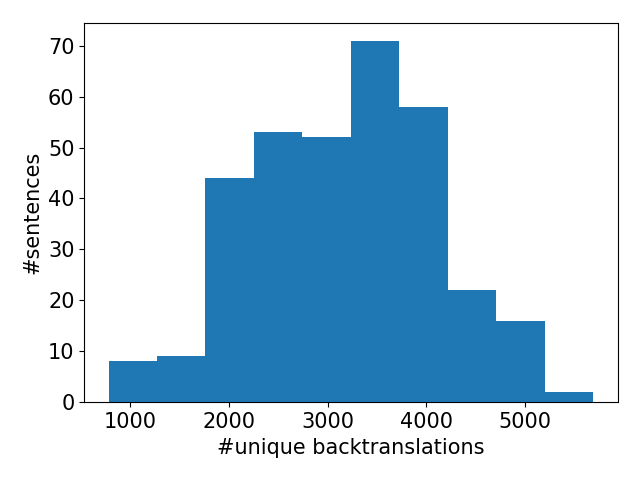
\includegraphics[width=\textwidth]{figures/uniqueness/unique_beam100/unique_back_original.png}
         \caption{Ambiguous Subset}
         %\label{fig:uniqueness_ambiguous}
     \end{subfigure}
     \hfill
     \begin{subfigure}{0.49\textwidth}
         \centering
         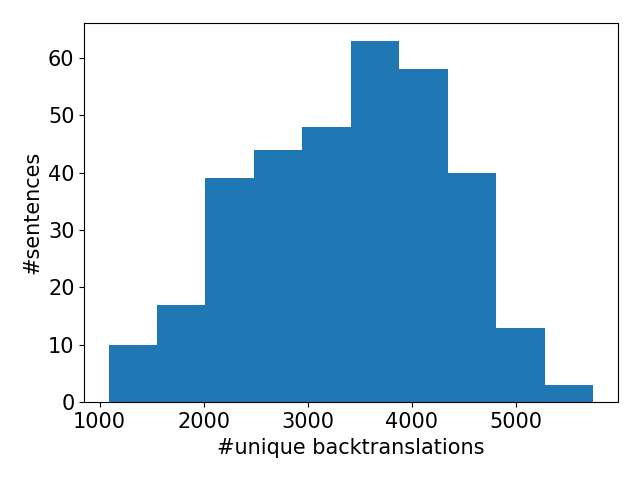
\includegraphics[width=\textwidth]{figures/uniqueness/unique_beam100/unique_back_male.png}
         \caption{Disambiguated Subset (male)}
         %\label{fig:uniqueness_male}
     \end{subfigure}
     \begin{subfigure}{0.49\textwidth}
         \centering
         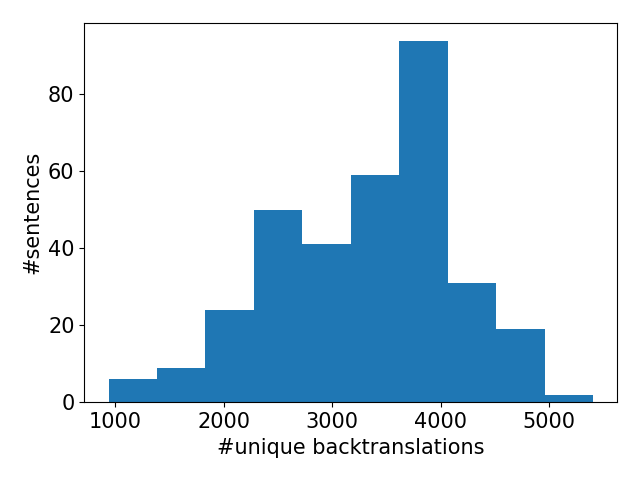
\includegraphics[width=\textwidth]{figures/uniqueness/unique_beam100/unique_back_average.png}
         \caption{Non-ambiguous Subset Average}
         %\label{fig:uniqueness_common}
     \end{subfigure}
     \hfill
     \begin{subfigure}{0.49\textwidth}
         \centering
         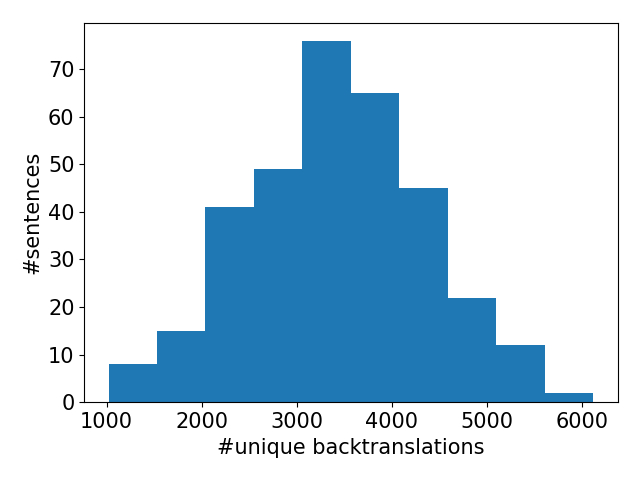
\includegraphics[width=\textwidth]{figures/uniqueness/unique_beam100/unique_back_female.png}
         \caption{Disambiguated Subset (female)}
         %\label{fig:uniqueness_female}
     \end{subfigure}
        \caption{Distribution of Unique Backtranslations: Beam search with beam size 100}
        \label{fig:uniqueness_graphs_100}

\end{figure}

\begin{figure}[!htb]
     \centering
     
     \begin{subfigure}{0.49\textwidth}
         \centering
         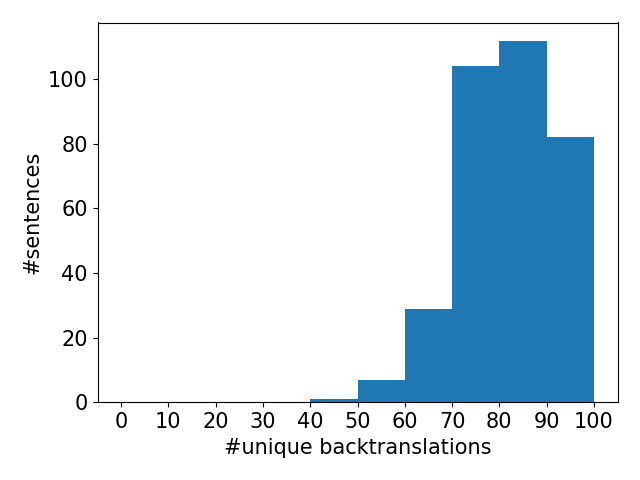
\includegraphics[width=\textwidth]{figures/uniqueness/unique_sampling/unique_back_original.png}
         \caption{Ambiguous Subset}
         %\label{fig:uniqueness_ambiguous}
     \end{subfigure}
     \hfill
     \begin{subfigure}{0.49\textwidth}
         \centering
         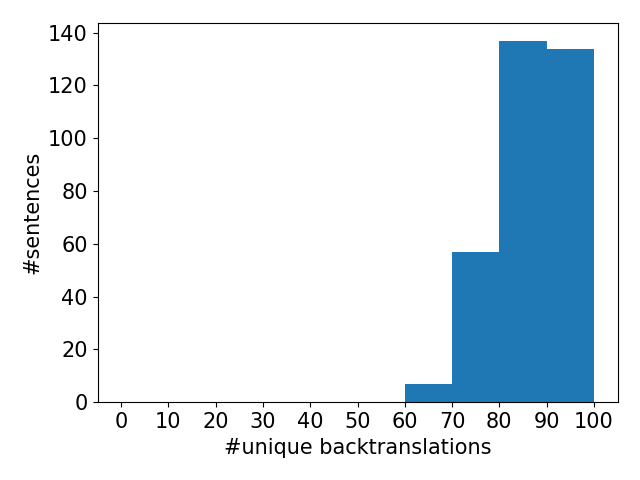
\includegraphics[width=\textwidth]{figures/uniqueness/unique_sampling/unique_back_male.png}
         \caption{Disambiguated Subset (male)}
         %\label{fig:uniqueness_male}
     \end{subfigure}
     \begin{subfigure}{0.49\textwidth}
         \centering
         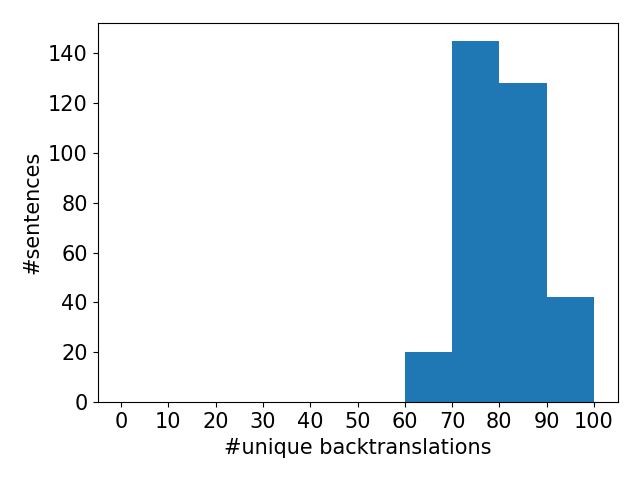
\includegraphics[width=\textwidth]{figures/uniqueness/unique_sampling/unique_back_average.png}
         \caption{Non-ambiguous Subset Average}
         %\label{fig:uniqueness_common}
     \end{subfigure}
     \hfill
     \begin{subfigure}{0.49\textwidth}
         \centering
         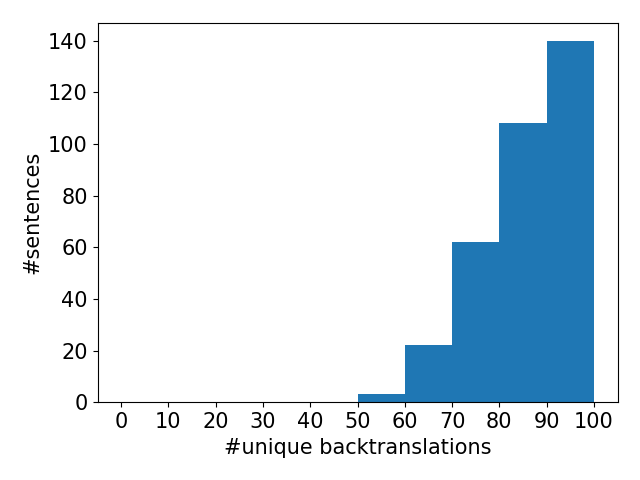
\includegraphics[width=\textwidth]{figures/uniqueness/unique_sampling/unique_back_female.png}
         \caption{Disambiguated Subset (female)}
         %\label{fig:uniqueness_female}
     \end{subfigure}
        \caption{Distribution of Unique Backtranslations: Sampling}
        \label{fig:uniqueness_graphs_sampling}

\end{figure}


%%%%%%%%%% Alignment distribution %%%%%%%%%%%%

% Beam 100
% Distribution for Translation
\begin{figure}[!htb]
     \centering
     
     \begin{subfigure}{0.49\textwidth}
         \centering
         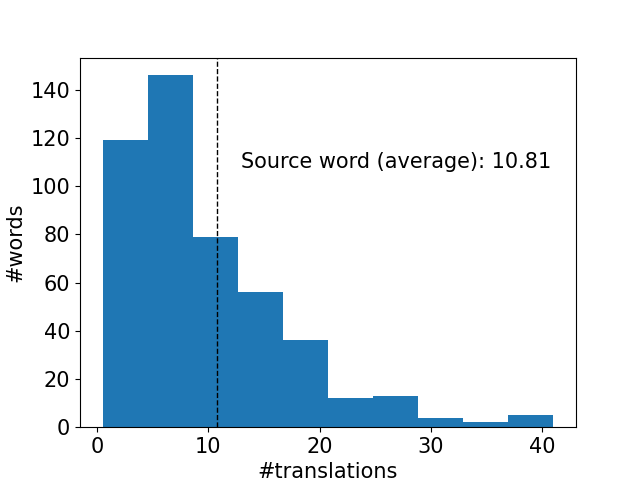
\includegraphics[width=\textwidth]{figures/alignment/align_100/word_translations_original.png}
         \caption{Ambiguous Subset}
         %\label{fig:alignment_translation_ambiguous}
     \end{subfigure}
     \hfill
     \begin{subfigure}{0.49\textwidth}
         \centering
         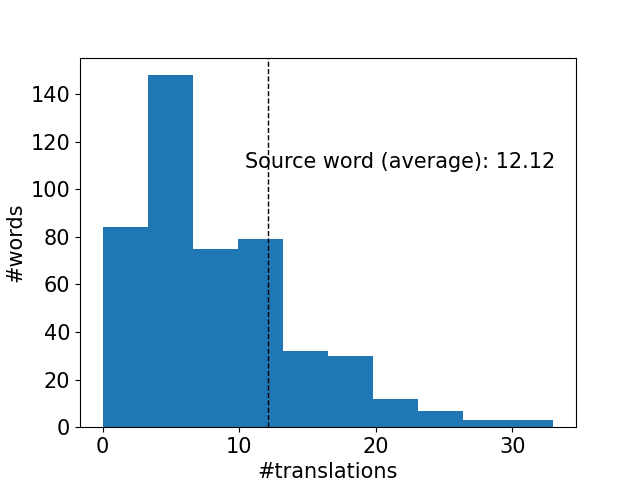
\includegraphics[width=\textwidth]{figures/alignment/align_100/word_translations_male.png}
         \caption{Disambiguated Subset (male)}
         %\label{fig:alignment_translation_male}
     \end{subfigure}
     \begin{subfigure}{0.49\textwidth}
         \centering
         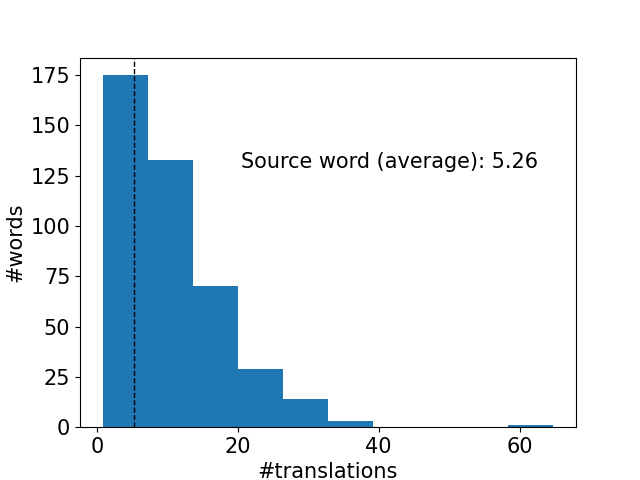
\includegraphics[width=\textwidth]{figures/alignment/align_100/word_translations_average.png}
         \caption{Non-ambiguous Subset Average}
         %\label{fig:alignment_translation_common}
     \end{subfigure}
     \hfill
     \begin{subfigure}{0.49\textwidth}
         \centering
         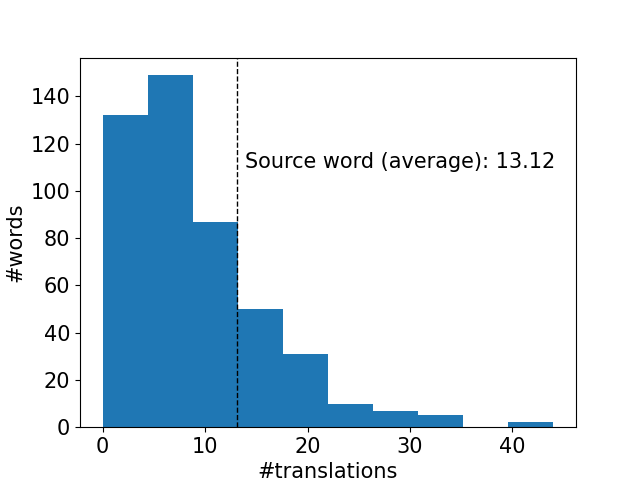
\includegraphics[width=\textwidth]{figures/alignment/align_100/word_translations_female.png}
         \caption{Disambiguated Subset (female)}
         %\label{fig:alignment_translation_female}
     \end{subfigure}
        \caption{\textbf{Distribution of Unique Translations for Words}. Beam search with beam size 100. Nbest size 100. Alignment with \textit{awesome-align}. The dashed line marks the average number of unique translations for the source word, the value displayed to the right.}
        \label{fig:alignment_graphs_translation_100}

\end{figure}

% Distribution for Backtranslation
\begin{figure}[!htb]
     \centering
     
     \begin{subfigure}{0.49\textwidth}
         \centering
         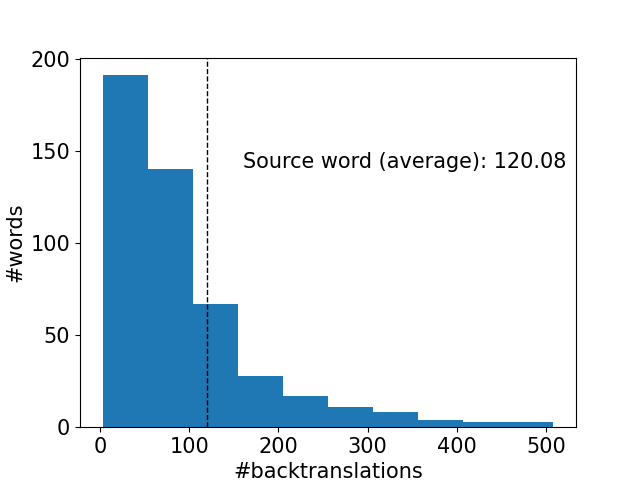
\includegraphics[width=\textwidth]{figures/alignment/align_100/word_backtranslations_original.png}
         \caption{Ambiguous Subset}
         %\label{fig:alignment_backtranslation_ambiguous}
     \end{subfigure}
     \hfill
     \begin{subfigure}{0.49\textwidth}
         \centering
         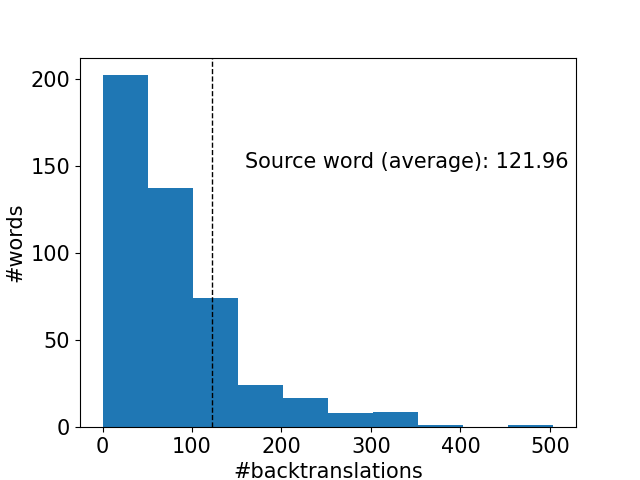
\includegraphics[width=\textwidth]{figures/alignment/align_100/word_backtranslations_male.png}
         \caption{Disambiguated Subset (male)}
         %\label{fig:alignment_backtranslation_male}
     \end{subfigure}
     \begin{subfigure}{0.49\textwidth}
         \centering
         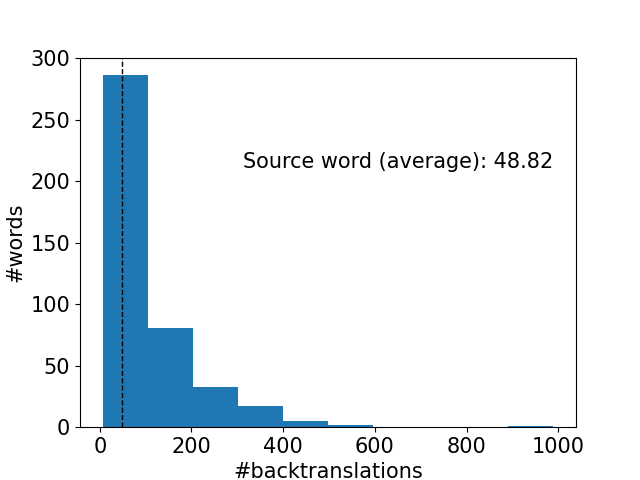
\includegraphics[width=\textwidth]{figures/alignment/align_100/word_backtranslations_average.png}
         \caption{Non-ambiguous Subset Average}
         %\label{fig:alignment_backtranslation_common}
     \end{subfigure}
     \hfill
     \begin{subfigure}{0.49\textwidth}
         \centering
         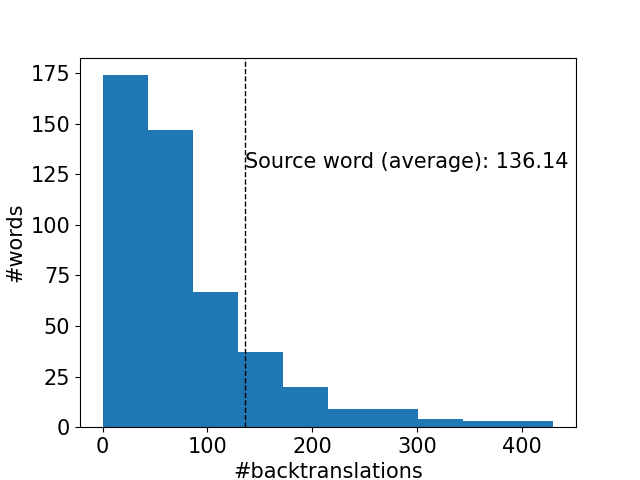
\includegraphics[width=\textwidth]{figures/alignment/align_100/word_backtranslations_female.png}
         \caption{Disambiguated Subset (female)}
         %\label{fig:alignment_backtranslation_female}
     \end{subfigure}
        \caption{\textbf{Distribution of Unique Backtranslations for Words}. Beam search with beam size 100. Nbest size 100. Alignment with \textit{awesome-align}. The dashed line marks the average number of unique translations for the source word, the value displayed to the right.}
        \label{fig:alignment_graphs_backtranslation_100}

\end{figure}

% Sampling
% Distribution for Translation
\begin{figure}[!htb]
     \centering
     
     \begin{subfigure}{0.49\textwidth}
         \centering
         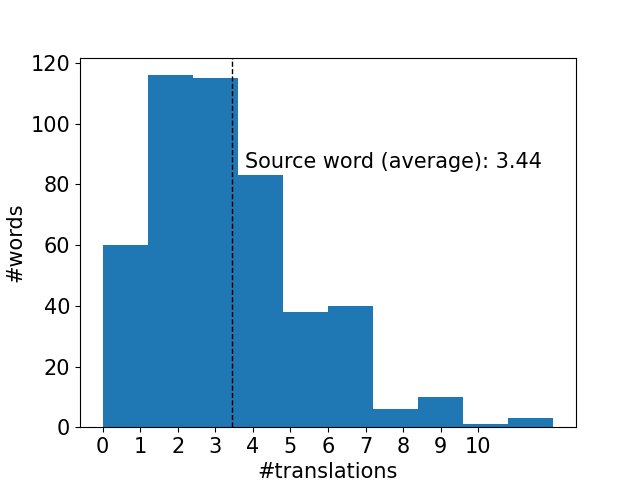
\includegraphics[width=\textwidth]{figures/alignment/align_sampling/word_translations_original.png}
         \caption{Ambiguous Subset}
         %\label{fig:alignment_translation_ambiguous}
     \end{subfigure}
     \hfill
     \begin{subfigure}{0.49\textwidth}
         \centering
         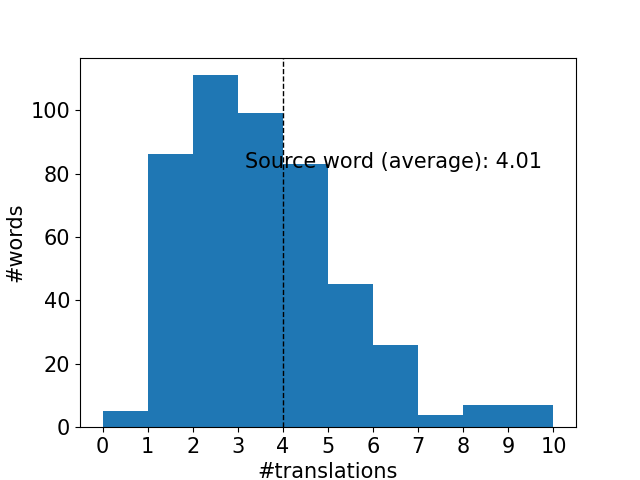
\includegraphics[width=\textwidth]{figures/alignment/align_sampling/word_translations_male.png}
         \caption{Disambiguated Subset (male)}
         %\label{fig:alignment_translation_male}
     \end{subfigure}
     \begin{subfigure}{0.49\textwidth}
         \centering
         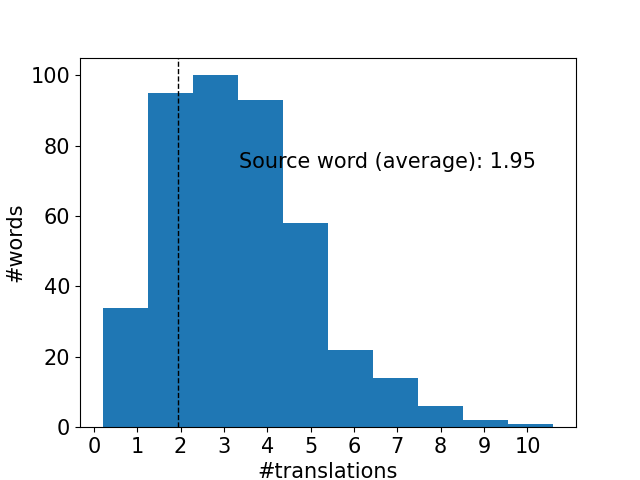
\includegraphics[width=\textwidth]{figures/alignment/align_sampling/word_translations_average.png}
         \caption{Non-ambiguous Subset Average}
         %\label{fig:alignment_translation_common}
     \end{subfigure}
     \hfill
     \begin{subfigure}{0.49\textwidth}
         \centering
         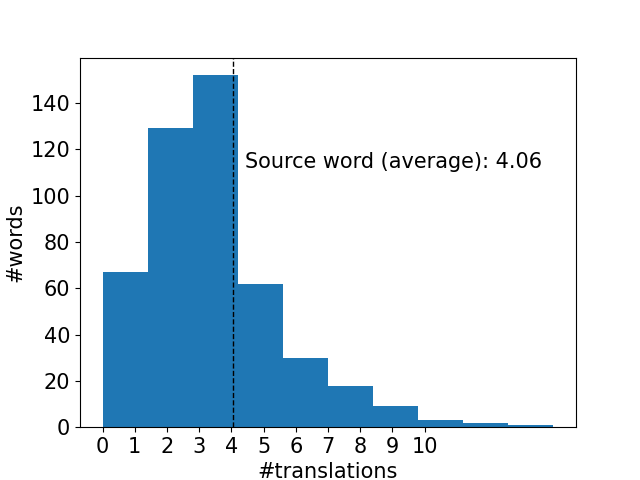
\includegraphics[width=\textwidth]{figures/alignment/align_sampling/word_translations_female.png}
         \caption{Disambiguated Subset (female)}
         %\label{fig:alignment_translation_female}
     \end{subfigure}
        \caption{\textbf{Distribution of Unique Translations for Words}. Sampling. Nbest size 10. Alignment with \textit{awesome-align}. The dashed line marks the average number of unique translations for the source word, the value displayed to the right.}
        \label{fig:alignment_graphs_translation_sampling}

\end{figure}

% Distribution for Backtranslation
\begin{figure}[!htb]
     \centering
     
     \begin{subfigure}{0.49\textwidth}
         \centering
         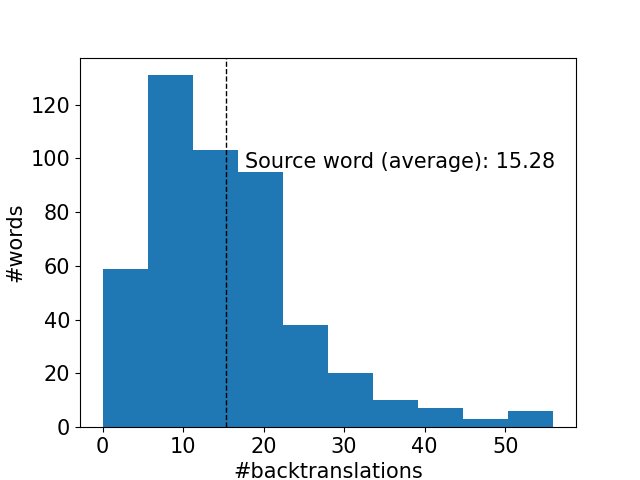
\includegraphics[width=\textwidth]{figures/alignment/align_sampling/word_backtranslations_original.png}
         \caption{Ambiguous Subset}
         %\label{fig:alignment_backtranslation_ambiguous}
     \end{subfigure}
     \hfill
     \begin{subfigure}{0.49\textwidth}
         \centering
         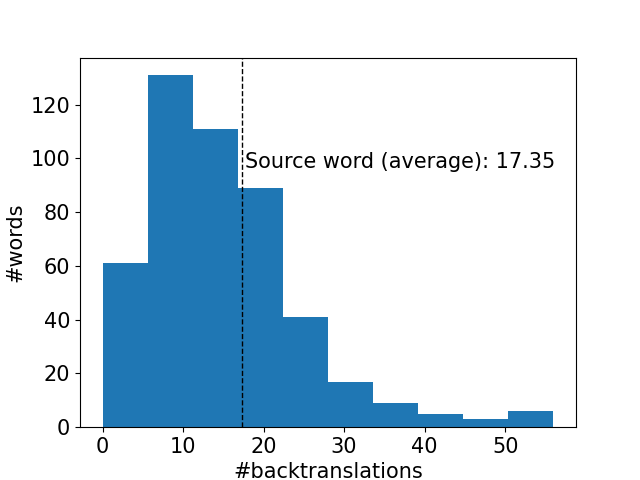
\includegraphics[width=\textwidth]{figures/alignment/align_sampling/word_backtranslations_male.png}
         \caption{Disambiguated Subset (male)}
         %\label{fig:alignment_backtranslation_male}
     \end{subfigure}
     \begin{subfigure}{0.49\textwidth}
         \centering
         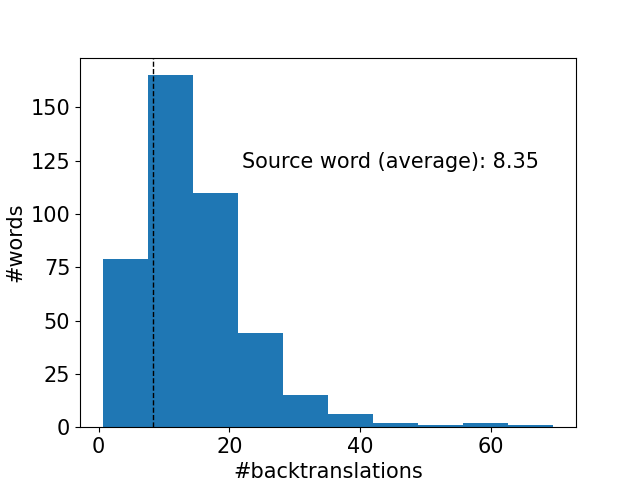
\includegraphics[width=\textwidth]{figures/alignment/align_sampling/word_backtranslations_average.png}
         \caption{Non-ambiguous Subset Average}
         %\label{fig:alignment_backtranslation_common}
     \end{subfigure}
     \hfill
     \begin{subfigure}{0.49\textwidth}
         \centering
         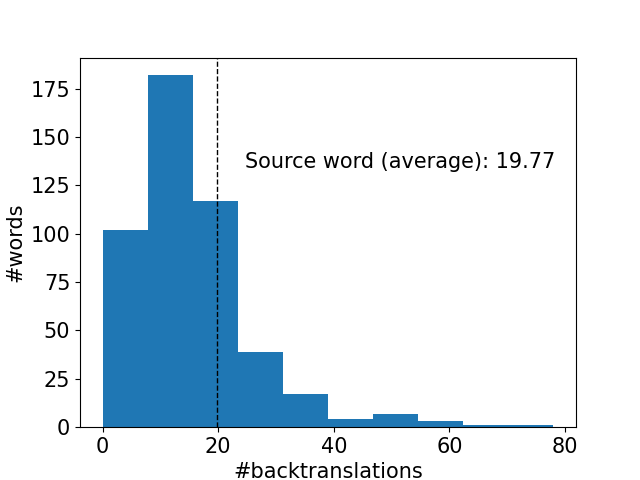
\includegraphics[width=\textwidth]{figures/alignment/align_sampling/word_backtranslations_female.png}
         \caption{Disambiguated Subset (female)}
         %\label{fig:alignment_backtranslation_female}
     \end{subfigure}
        \caption{\textbf{Distribution of Unique Backtranslations for Words}. Sampling. Nbest size 10. Alignment with \textit{awesome-align}. The dashed line marks the average number of unique translations for the source word, the value displayed to the right.}
        \label{fig:alignment_graphs_backtranslation_sampling}

\end{figure}

\end{document}
